\begin{frame}
	\myheading{Module 5.3 : Contours}
\end{frame}

\begin{frame}
	\fontsize{16pt}{7.2}\selectfont
	\begin{itemize}\justifying
		\item \textit{Visualizing things in 3d can sometimes become a bit cumbersome}
		      \item<2-> \textit{Can we do a 2d visualization of this traversal along the error surface}
		      \item<3-> \textit{Yes, let's take a look at something known as contours}
	\end{itemize}
	 
\end{frame}

\begin{frame}
	\begin{columns}
		\column{0.5\textwidth}
		\begin{overlayarea}{\textwidth}{\textheight}
			\begin{figure}
				\begin{tikzpicture}
\begin{axis}[axis lines=left, ticks=none,xmax=0.5,ymax=0.5,x label style={at={(axis description cs:0.5,0)},anchor=north},
xlabel={$\theta$}, ylabel={error}]
\addplot[thick,black, no markers, samples=200, domain=-5:0] {-x*exp(x)};
\only<2->{\draw[dashed] (axis cs:-1.88,0.31) -- (axis cs:-0.0,0.31)} ;
\only<2->{\draw[dashed] (axis cs:-2.68,0.21) -- (axis cs:-0.0,0.21)} ;

\end{axis}
\end{tikzpicture}

				\caption{Front view of a 3d error surface}
				
			\end{figure}
		\end{overlayarea}
		
		\column{0.5\textwidth}
		\begin{overlayarea}{\textwidth}{\textheight}
			\only<1-2>{
				\begin{itemize}\justifying
					\item Suppose I take horizontal slices of this error surface at regular intervals along the vertical axis
					\item <2>How would this look from the top-view ?
				\end{itemize}
			}
			
			\only<3->{
				\tikzstyle{neuron}=[circle,draw=blue!50,fill=blue!20,thick,minimum size=10mm]
\tikzstyle{input}=[circle,draw=black!50,fill=black!20,thick,minimum size=6mm]
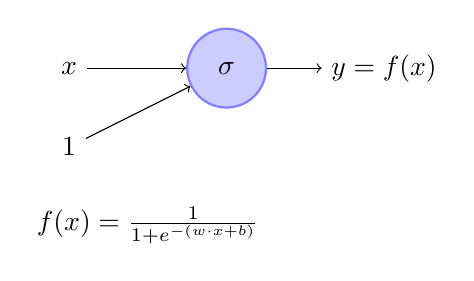
\begin{tikzpicture}
\node [neuron] (neuron0) at (1,6)  {$\sigma$} ;
\node (input1) at (-1,6)  {$x$};
\node (input0) at (-1,5)  {$1$};
\node (output0) at (3,6)  {$y = f(x)$};
\node (formula) at (0,4) {$f(x)= \frac{1}{1+e^{-(w\cdot x + b)}}$};
\draw [->] (input0) -- (neuron0);
\draw [->] (input1) -- (neuron0);
\draw [->] (neuron0) -- (output0);
\end{tikzpicture}

				\begin{itemize}\justifying
					\item<4-> A small distance between the contours indicates a steep slope along that direction
					\item<5-> A large distance between the contours indicates a gentle slope along that direction
				\end{itemize}
			}
			
		\end{overlayarea}
	\end{columns}
	
\end{frame}

\begin{frame}
	\fontsize{16pt}{7.2}\selectfont
	\begin{itemize}\justifying
		\item \textit{Just to ensure that we understand this properly let us do a few exercises ...}
	\end{itemize}
	 
\end{frame}


\begin{frame}
	\begin{columns}
		\column{0.5\textwidth}
		\begin{overlayarea}{\textwidth}{\textheight}
			\begin{figure}
				\includegraphics<1-2>[scale=0.4]{images/module3/trial/2d_43.png}
				\includegraphics<3-4>[scale=0.4]{images/module3/trial/2d_34.png}
				\includegraphics<5->[scale=0.4]{images/module3/trial/2d_32.png}
			\end{figure}
			\only<1->{Guess the 3d surface}
		\end{overlayarea}
		
		\column{0.5\textwidth}
		\begin{overlayarea}{\textwidth}{\textheight}
			\begin{figure}
				\includegraphics<2>[scale=0.5]{images/module3/trial/3d_43.png}
				\includegraphics<4>[scale=0.5]{images/module3/trial/3d_34.png}
				\includegraphics<6>[scale=0.5]{images/module3/trial/3d_32.png}
			\end{figure}
		\end{overlayarea}
	\end{columns}
	
\end{frame}



\begin{frame}
	\fontsize{16pt}{7.2}\selectfont
	\begin{itemize}\justifying
		\item \textit{Now that we know what are contour maps and how to read them let us go back to our toy example and visualize gradient descent from the point of view of contours...}
	\end{itemize}
	 
\end{frame}


\begin{frame}
	\begin{columns}
		\column{0.5\textwidth}
		\begin{overlayarea}{\textwidth}{\textheight}
			\begin{figure}
				\foreach \n in {0,...,50} {%
					\begin{tikzpicture}
						\sbox0{%
						\includegraphics[scale=0.4]{images/module3/sgd0/sgd_quiver\n.png}
						}%
						\only<\n>{\node[above right,inner sep=0pt] at (0,0)  {\usebox{0}}};%
						\only<\n>{\node[red,font=\small](w) at (0.5\wd0,0.23\ht0) {w}};%
						\only<\n>{\node[red,font=\small](b) at (0,0.67\ht0) {b}};%
						\only<\n>{\draw[->, line width=0.2mm](w)--(0.6\wd0,0.23\ht0)};%
						\only<\n>{\draw[->, line width=0.2mm](b)--(0,0.8\ht0)};%
					\end{tikzpicture}
				}%
			\end{figure}
		\end{overlayarea}
		
		\column{0.5\textwidth}
		\begin{overlayarea}{\textwidth}{\textheight}
			
			\begin{figure}
				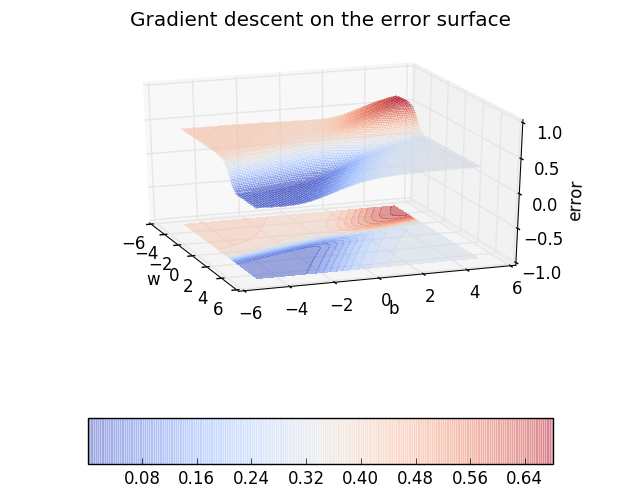
\includegraphics[scale=0.5]{images/module3/sgd0/sgd_error_with_contour.png}
			\end{figure}
			
			
		\end{overlayarea}
	\end{columns}
	
\end{frame}

\begin{frame}
	\begin{columns}
		\column{0.5\textwidth}
		\begin{overlayarea}{\textwidth}{\textheight}
			\begin{figure}
				\foreach \n in {0,...,29} {%
					\pgfmathtruncatemacro\result{int(round(\n+50))}
					\begin{tikzpicture}
						\sbox0{%
						\includegraphics[scale=0.4]{images/module3/sgd0/sgd_quiver\result.png}
						}%
						\only<\n>{\node[above right,inner sep=0pt] at (0,0)  {\usebox{0}}};%
						\only<\n>{\node[red,font=\small](w) at (0.5\wd0,0.23\ht0) {w}};%
						\only<\n>{\node[red,font=\small](b) at (0,0.67\ht0) {b}};%
						\only<\n>{\draw[->, line width=0.2mm](w)--(0.6\wd0,0.23\ht0)};%
						\only<\n>{\draw[->, line width=0.2mm](b)--(0,0.8\ht0)};%
					\end{tikzpicture}
				}%
			\end{figure}
		\end{overlayarea}
		
		\column{0.5\textwidth}
		\begin{overlayarea}{\textwidth}{\textheight}
			
			\begin{figure}
				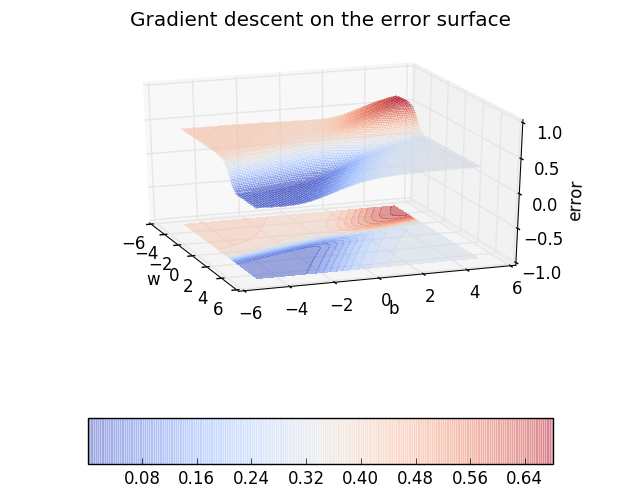
\includegraphics[scale=0.5]{images/module3/sgd0/sgd_error_with_contour.png}
			\end{figure}
			
			
		\end{overlayarea}
	\end{columns}
	
\end{frame}
